\documentclass[hyperref={pdfpagelabels=false}]{beamer}

\usecolortheme{crane}
\usepackage{wrapfig}
\usepackage{lmodern}

\usepackage{natbib}
\usepackage{amsmath,amsfonts,amssymb}

\usepackage{algorithm,algorithmic}
\floatname{algorithm}{Algorithmus}

\usepackage{wrapfig}
\usepackage{xcolor}


\usepackage[english]{babel}

\usepackage{hyperref}
\usepackage{graphicx}
\definecolor{darkred}{rgb}{110,1,1}  
\definecolor{maroon}{rgb}{0.5,0,0}  

\newcounter{saveenumi}
\newcommand{\seti}{\setcounter{saveenumi}{\value{enumi}}}
\newcommand{\conti}{\setcounter{enumi}{\value{saveenumi}}}

\renewcommand{\algorithmicforall}{\textbf{for each}}

\title{{P}rogressive {G}raph {M}atching:\\
		{M}aking a {M}ove of {G}raphs via {P}robabilistic {V}oting}   
\author{Minsu Cho\\
		Kyoung Mu Lee\\
		\vspace{20pt}
		Proc. Computer Vision and Pattern Recognition (CVPR) \text{2012}}
\date{}

\usepackage{beamerthemeshadow}

\renewcommand{\thefootnote}{\fnsymbol{footnote}} 


\begin{document}

%--------------------------------------------------------------------------%
\begin{frame}
\titlepage
\end{frame}
%--------------------------------------------------------------------------%
\begin{frame}
\frametitle{Graph Matching}
Given two attributed graphs $\bar{G}^P=(\bar{V}^P, \bar{E}^P, \bar{A}^P)$ and $\bar{G}^Q=(\bar{V}^Q, \bar{E}^Q, \bar{A}^Q)$ with $n^P$ and $n^Q$ nodes respectively.

A result of graph matching is a subset of possible correspondences between those graphs, which can be represented in form of assignment matrix $X\in\{0,1\}^{n^P\times n^Q}$:
$$X_{ia} = \begin{cases} 1 & \mbox{node}\ v_i\in \bar{V}^P \mbox{matches}\ v_a \in \bar{V}^Q \\
						 0 & \mbox{otherwise} \\
			\end{cases}$$
General formulation:
$$x^* = \arg\max S(x)$$
$$ s.t. \begin{cases}
									x\in{0,1}^{n^Pn^Q} \\
								 \sum_{i=1}^{n^P}x_{ia}\le 1 \\
								 \sum_{a=1}^{n^Q}x_{ia}\le 1  \end{cases}$$
The objective function $S(x)$ measures the similarity between the graph attributes. 
\end{frame} 

%--------------------------------------------------------------------------%
\begin{frame}
\frametitle{Integer Quadratic Programming}

Consider two types of similarity: node and edge similarity. Those can be combined in an affinity matrix $W$, where non-diagonal elements $W_{ia,jb}$ represent edge similarity of the edges $e_{ij}\in \bar{E}^P$ and $e_{ab}\in \bar{E}^Q$ and diagonal elements $W_{ia,ia}$ represent similarity between nodes $v_i\in \bar{V}^P$ and $v_a\in \bar{V}^Q$.

That leads to the integer quadratic optimization problem:\\
$$x^* = \arg\max x^TWx\ $$
$$\mbox{s.t}. \begin{cases}
					x\in{0,1}^{n^Pn^Q} \\
					\sum_{i=1}^{n^P}x_{ia}\le 1 \\
					\sum_{a=1}^{n^Q}x_{ia}\le 1  \end{cases}$$
\end{frame}

\begin{frame}
\frametitle{Issues}
\begin{itemize}
\item Quadratic assignemnt problem is $NP$-complete
\item Computation of $W$ for a large graph is almost infeasible
\item Reduction of the complexity often leads to worse matching results
\end{itemize}
\end{frame}

\begin{frame}
\frametitle{Progressive Graph Matching}
Refer to the initial graphs $\bar{G}^P$ and $\bar{G}^Q$ as \textcolor{red}{maximal graphs}. 
For each maximal graph a subgraph induced by a reduced set of nodes is called \textcolor{red}{active graph} ($G^P$ and $G^Q$ respectively).

\vspace{10pt}
Idea: match maximal graphs by iteratively matching their active graphs ($t=0,1,\dots$)
\begin{itemize}
\item \textcolor{red}{Graph Matching}\\
		match current active graphs $G_t^P=(V_t^P, E_t^P, A_t^P)$ and $G_t^Q=(V_t^Q, E_t^Q, A_t^Q)$, $G_t^P\subset \bar{G}^P$,$G_t^Q\subset \bar{G}^Q$.
\item \textcolor{red}{Graph Progression}\\
		update active graphs to improve matching score on the next matching step
\end{itemize}

\end{frame}

\begin{frame}
\frametitle{Graph Matching}
To reduce the complexity of graph matching consider a given \textcolor{red}{set of candidate matches} $C_t\subset V^P\times V^Q$.

The corresponding active graphs are defined by the nodes appeared in $C_t$.

This method reduces the size of active graphs and makes a affinity matrix more sparse.

\end{frame}

\begin{frame} [allowframebreaks]
\frametitle{Graph Progression}
Let $M_t=\{m_1,\dots,m_{|M_t|}\}\subset C_t$ with $m_i=(v_{p_i}^P,v_{q_i}^Q)$ be a \textcolor{red}{result of graph matching} of two active graphs and $s_t$ it's \textcolor{red}{score}.

Consider conditional joint probability \textcolor{red}{$p(V^P,V^Q|M_t)$}:
\begin{align*}
	p(V^P,V^Q|M_t) = \sum_{m_i\in M_t}& p(V^P,V^Q,M=m_i|M_t) \\
				   = \sum_{m_i\in M_t}& p(V^Q|V^P,M=m_i,M_t)\\
				   & p(V^P|M=m_i, M_t) p(M=m_i|M_t)\\
\end{align*}

\framebreak

$p(v_i^P,v_a^Q|M_t)$	conditional probability of match $(v_i^P,v_a^Q)$ between two maximal graphs.

Base on the probability distribution $p(V^P,V^Q|M_t)$ new candidate set $C_{t+1}$ consists of $N_c$ best matches. 

Given new candidate set $C_{t+1}$ we obtain new active graphs $G_{t+1}^P$ and $G_{t+1}^P$.

The condition $M_t\subset C_{t+1}$ ensures that $s_{t+1}\ge s_t$, if $M_t$ is an optimal matching. 

\end{frame}

\begin{frame}
\frametitle{Algorithm}

\begin{algorithm}[H]
	\fontsize{9pt}{6}\selectfont
				\begin{algorithmic}[1]
				
				\STATE $C_0=Find\_Initial\_Candidates(\bar{G}^P, \bar{G}^Q, N_c)$
				\STATE $t=0, s_0 = 0$
				\WHILE{$\mbox{score increases}$}
					\STATE $(M_t,s_t)=Graph\_Matching(C_t)$ 
					\STATE $p(v_p^P,v_q^Q|M_t)=0\ \ \forall v_p^P\in \bar{V}^P, v_q^Q\in \bar{V}^Q$
					\FORALL{$m_i=(v_p^P,v_q^Q)\in M_t$}
						\STATE $N_A=\{v^P\in \bar{V}^Q| p(v^P|m_i, M_t)>\epsilon\}$
						\FORALL{$v_j^P\in N_A$}
							\STATE $N_B=\{v^Q\in \bar{V}^Q| p(v^Q|v_j^P, m_i, M_t)>\epsilon\}$
							\FORALL{$v_b^Q\in N_b$}
								\STATE $p(v_p^P,v_q^Q|M_t)=p(v_p^P,v_q^Q|M_t)+
								p(v_b^Q|v_j^P, m_i,M_t)p(v_j^P|m_i,M_t)p(m_i|M_t)$
							\ENDFOR
						\ENDFOR
					\ENDFOR
					\STATE $C_{t+1}=N_c\ \mbox{best matches based on}\  p(V^P,V^Q|M_t)\mbox{, which contains}\ M_t$
					\STATE $t=t+1$
				\ENDWHILE
				\RETURN $M_t$
				
				\end{algorithmic}
				\caption{progressiveGraphMatching($\bar{G}^P$, $\bar{G}^Q$, $N_c$) \cite{MinsuCho}}
			\end{algorithm}
	\end{frame}
%-----------------------------------------------------------------------------
\begin{frame}[allowframebreaks]
\frametitle{Matching of images}
Given two images.
\begin{itemize}
\item Detected features of the images represent nodes of the maximal graphs (and their geometric relations as edges)
\item Node similarity  = similarity of feature descriptors of two graphs
\item Edge similarity = Symmetric Transfer Error (STE) (see \cite{MinsuChoRRW})
\end{itemize}

\begin{columns}[T]
\fontsize{10pt}{6}\selectfont
	\begin{column}{0.6\textwidth}
		Derive affine homography transformation $\tau_{ia}(\cdot)$ between two features\\
		\vspace{10pt}
		The transfer error of $(j,b)$ with respect to $(i,a)$
		$$d_{jb|ia}=\|x_b^Q-\tau_{ia}(x_j^P)\|$$\\
		Edge similarity $W_{ia,jb} = \max(0, \alpha - \frac{d_{jb|ia}+d_{bj|ai}+d_{ia|jb}+d_{ai|jb}}{4} )$
	\end{column}
	\begin{column}{0.4\textwidth}
		\begin{figure}
			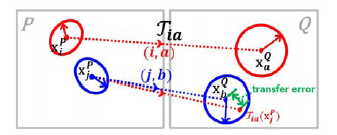
\includegraphics[scale=0.5]{fig4.png}
		\end{figure}
	\end{column}
\end{columns}
	

\framebreak

\fontsize{7pt}{6}\selectfont

$$ \mathbf{p(V^P,V^Q|M_t) = \sum_{m_i\in M_t}p(V^Q|V^P,M=m_i,M_t)p(V^P|M=m_i, M_t)p(M=m_i|M_t)}$$

\begin{itemize}
  \begin{columns}[T]
    \begin{column}{0.75\textwidth}
	\item $\mathbf{p(M=m_i|M_t)} = score(m_i)/\sum_i score(m_i)$\\
    \end{column}
    
    \begin{column}{0.3\textwidth}
    \end{column}
  \end{columns}


  \begin{columns}[T]
    \begin{column}{0.75\textwidth}
	\item Assuming $m_i=(v_{p_i}^P,v_{q_i}^Q)$ and use function $kNN(\cdot,k)$ to find $k$-nearest neighbors of a node\\
		$$\mathbf{p(V^P=v_j^P|M=m_i,M_t)} = \begin{cases}
			1/k_{1} &, \ \mbox{if}\ v_j^P\in kNN(v_{p_i}^P, k_1)\\
			0 &, \ \mbox{otherwise}
		\end{cases}$$
    \end{column}
    
    \begin{column}{0.3\textwidth}
	\begin{figure}
	  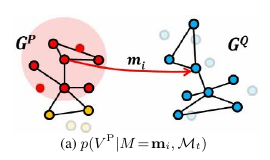
\includegraphics[scale=0.5]{fig3a.png}
	\end{figure}
    \end{column}
  \end{columns}

  \begin{columns}[T]
    \begin{column}{0.75\textwidth}
	\item Let $NN(\cdot)$ define a nearest neighbor of a node\\
	      \vspace{10pt}
	      $$\mathbf{p(V^Q=v_b^Q|V^P=v_j^P,M=m_i,M_t)} = $$
	      $$\begin{cases}
		  1 &,\ \mbox{if}\ v_b^Q =NN(\tau_{m_i}(p_j^P))\ \mbox{and}\ (v_j^P,v_b^Q)\in M_t\\
		  \exp(-d_{jb|mi})/Z &,\ \mbox{if}\ v_b^Q\in kNN(\tau_{m_i}(p_j^P),k_2)\ \mbox{and}\ (v_j^P,NN(\tau_{m_i}(p_j^P)))\not\in M_t \\
		  0 &,\ \mbox{otherwise}
		\end{cases}$$
    \end{column}
    
    \begin{column}{0.3\textwidth}
	\begin{figure}
	  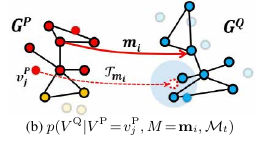
\includegraphics[scale=0.5]{fig3b.png}
	\end{figure}
    \end{column}
  \end{columns}

\end{itemize}

$Z = \sum_{v_b^Q\in kNN(\tau_{m_i}(p_j^P),k_2)}\exp(-d_{jb|mi})$ is a normalization constant

\end{frame}


%\begin{frame}
%\frametitle{Complexity}

%Each iteration of the algorithm can be performed  in %$O(k_1k_2|M_t|log(|\bar{V}^P|)log(|\bar{V}^Q|))$

%\end{frame}
%-----------------------------------------------------------------------------
\begin{frame}
\frametitle{Evaluation}

\begin{itemize}
 \item Parameters of the affinity matrix $W$: $\mathbf{\alpha = 50}$, $\mathbf{k_1=25}$, $\mathbf{k_2=5}$
 \item Used Descriptors: {\bf MSER} \cite{MSER} and Harris-affine and Hessian-affine features \cite{HarrisAffine}
 \item used graph mathing methonds: \\
      Graduate Assigment Algorithm ({\bf SM}) \cite{SM} \\
      Spectral Matching with Affine Constraint ({\bf SMAC}) \cite{SMAC} \\
      Probabilistic Graph Matching ({\bf PM}) \cite{PM}\\
      Reweighted Random Walk Method ({\bf RRWM})\cite{MinsuChoRRW}\\
      Integer Projected Fixed Point Method ({\bf IPFP}) \cite{IPFP}
  \item Datasets: {\bf VOC 2010}, {\bf Caltech-101}, {\bf MSRC}, {\bf ETHZ} toys dataset   
   
\end{itemize}

\end{frame}

\begin{frame}
\frametitle{Evaluation: Progressive Graph Matching ($N_c=1000$)}
\begin{figure}
  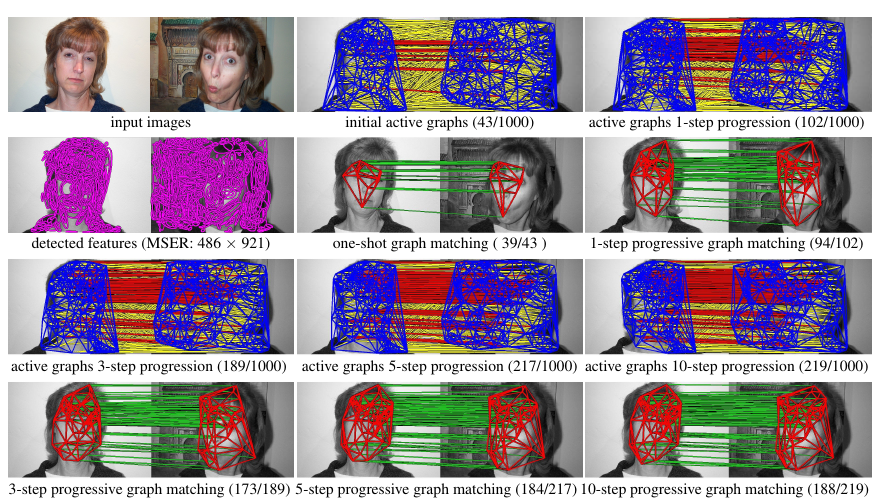
\includegraphics[scale=0.5]{fig1sub.png}
\end{figure}
\end{frame}

\begin{frame}
\frametitle{Evaluation: Progressive Graph Matching ($N_c=3000$)}
\begin{figure}
  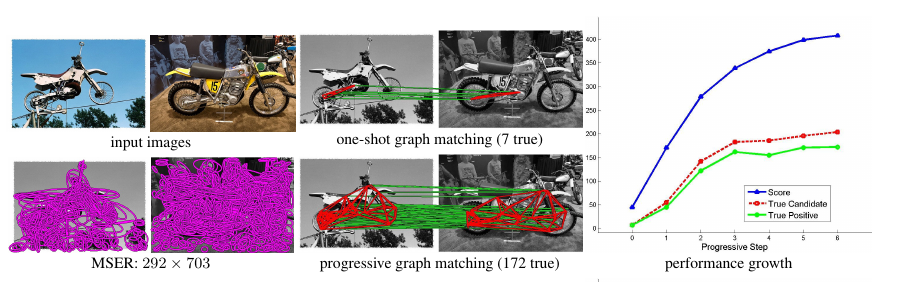
\includegraphics[scale=0.5]{fig3asub.png}
\end{figure}
\end{frame}

\begin{frame}
\frametitle{Evaluation: Progressive Graph Matching ($N_c=3000$)}
\begin{figure}
  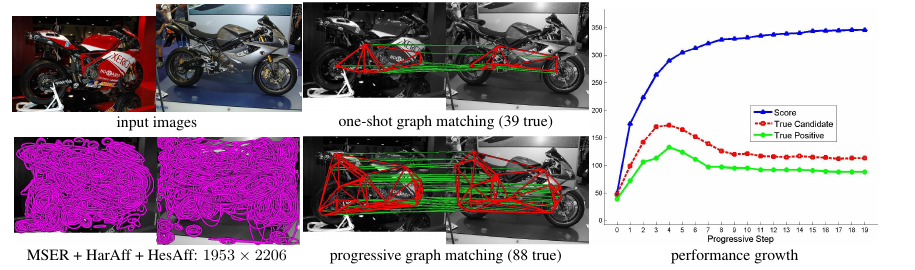
\includegraphics[scale=0.5]{fig3csub.png}
\end{figure}
\end{frame}

\begin{frame}
\frametitle{Evaluation: Progressive Graph Matching ($N_c=3000$)}
\begin{figure}
  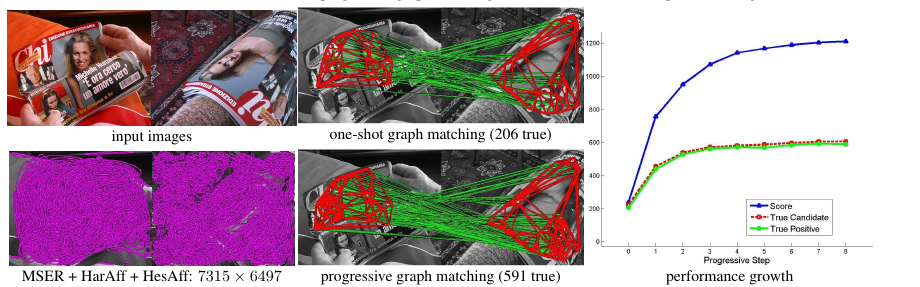
\includegraphics[scale=0.5]{fig6csub.png}
\end{figure}
\end{frame}


\begin{frame}[allowframebreaks]
\frametitle{Evaluation: Robustness to initial active graph ($N_c=3000$)}
\begin{figure}
  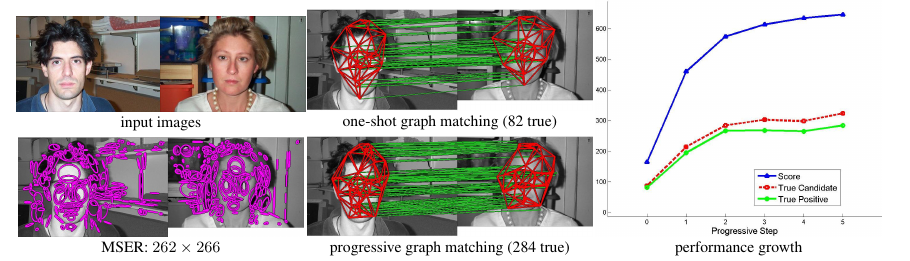
\includegraphics[scale=0.5]{fig7asub.png}
\end{figure}

\framebreak

\begin{figure}
  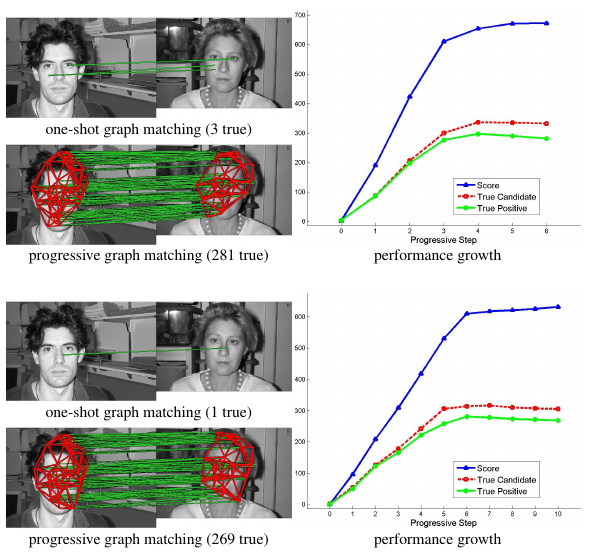
\includegraphics[scale=0.5]{fig7bcsub.png}
\end{figure}
\end{frame}

\begin{frame}
 \frametitle{Evaluation: Different matching algorithms}
 \begin{figure}
  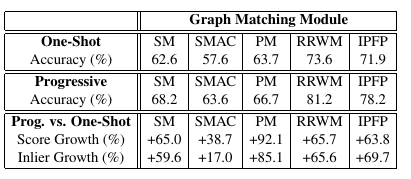
\includegraphics[scale=0.8]{fig_table1.png}
  \caption{Dataset of $30$ image pairs. Accuracy boost $3\%\sim 8\%$}
 \end{figure}

\end{frame}


%-----------------------------------------------------------------------------
\begin{frame}
 \frametitle{Conclusions}
 \begin{itemize}
  \item graph progression significantly increases one-step graph matching
  \item algorithm is suitable for large graphs
  \vspace{30pt}
  
  \item (?) convergense of the algorithm
  \item (?) selection of the candidate matches
  \item (?) number of the candidate matches
  \item (?) running time
  \item (?) geometric graphs
 \end{itemize}

\end{frame}

%-----------------------------------------------------------------------------
\begin{frame}{The End}
\centering
\LARGE
\color{red}
 Thank you for your attention!
 
 \nocite{MinsuChoSubb}
\end{frame}

%-----------------------------------------------------------------------------
\begin{frame} [allowframebreaks]
	\frametitle{References}
	\bibliographystyle{plain}
	\bibliography{bibliographie}
\end{frame} 

\end{document}
